\chapter{Stakeholder Security Analysis}
\section{Introduction}
\thispagestyle{empty}
\pagestyle{empty}
% The very first letter is a 2 line initial drop letter followed
% by the rest of the first word in caps.
% 
% form to use if the first word consists of a single letter:
% \PARstart{A}{demo} file is ....
% 
% form to use if you need the single drop letter followed by
% normal text (unknown if ever used by IEEE):
% \PARstart{A}{}demo file is ....
% 
% Some journals put the first two words in caps:
% \PARstart{T}{his demo} file is ....
% 
% Here we have the typical use of a "T" for an initial drop letter
% and "HIS" in caps to complete the first word.

%\PARstart{V}{ulnerabilities} of web systems take a great variety of forms

Cybersecurity issues and ethics  take a great variety of forms and new ones appear to emerge regularly, so it can seem an endless process to manage and maintain the cyber spase \cite{josang2005user}. An approach used periodically is to assign the task of attack or harm   a service in cyber space  to an individual or a team and then address the discovered weaknesses. We call this a {\em security audit}. The approach of searching for weaknesses and fixing them is so widely used that it might reasonably be regarded as a design philosophy.
This approach has been used in this dissertation, and the results of
both the attacks and the resulting defences are reported.
However, this approach is somewhat pessimistic in that it {\em assumes}
that a more methodical security design philosophy which can guarantee
secure design is not available. The main result
of this dissertation is to demonstrate such a methodical design philosophy.
We call this {\em stakeholder security analysis}.

Stakeholder security analysis proceeds as follows: 
\begin{enumerate}[1.]
\item Identify the key stakeholders.
\item For each stakeholder, identify a set of rules {\em required}
by these stakeholders. Note: the collected rules required
by all stakeholders must be consistent.
\item Implement procedures which ensure that all rules are enforced.
\end{enumerate}

Both a security audit and a stakeholder security analysis
are applied in this dissertation to a specific subsystem of a web
service system being developed and managed by the authors.
Note: it is not suggested that stakeholder security analysis obviates
the need for a security audit.

\subsection{The Netml System}
\begin{figure}
	\centering
		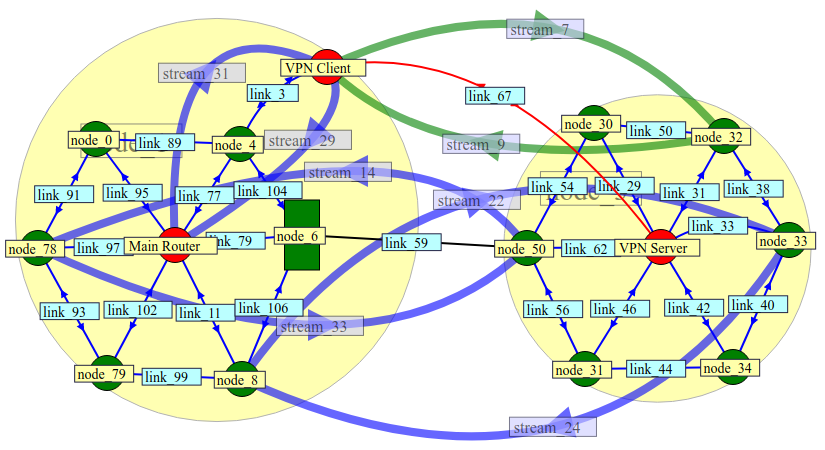
\includegraphics[width=6cm]{figures/vpn.png}
\caption{Two corporate networks }
\label{corporatenetwork}
\end{figure}

\begin{figure}
	\centering
		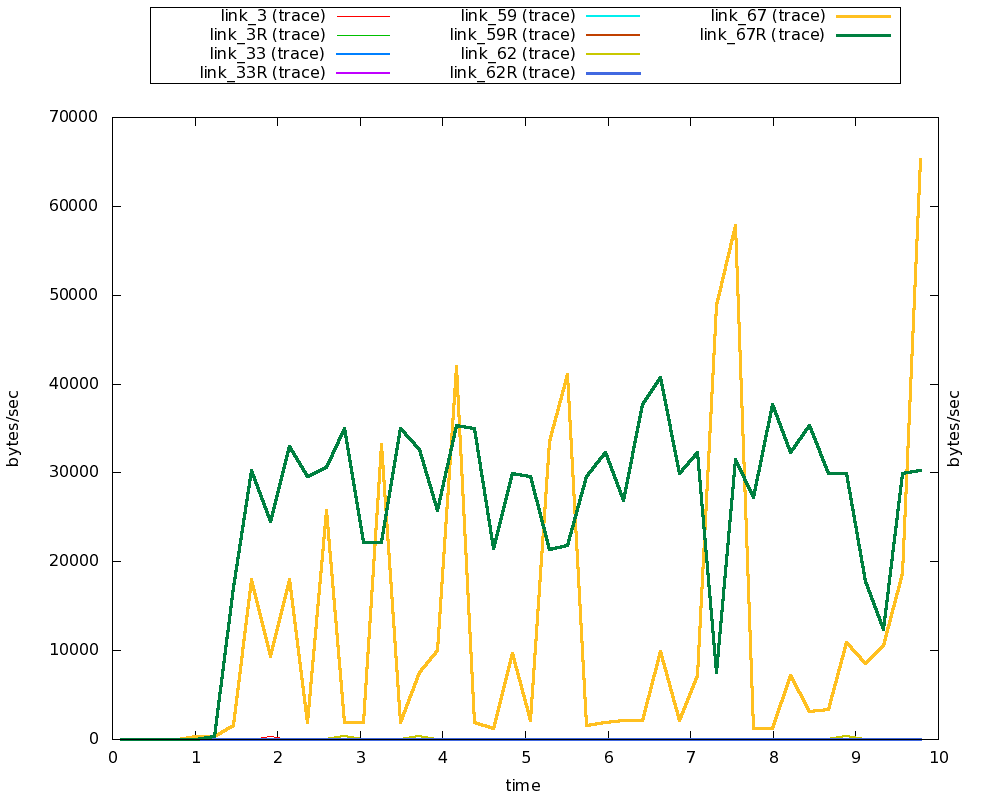
\includegraphics[width=6cm]{figures/vpn_traffic.png}
\caption{Traffic traces}
\label{Traffictraces}
\end{figure}

The Netml system provides services for analysis, design, and implementation
of networks \cite{addie2011netml}. These services are provided by means of a web
site Figure \ref{corporatenetwork}. No software is installed on users' computers (except in the form
of cached javascript). This system is used in teaching, by
computer science students, and in research into network analysis and design Figure  \ref{Traffictraces}. 
\iflonger
Most of the users of the Netml system, do not use it for an extended period of
time and therefore do not develop complex networks which incorporate a significant
investment. However, the security requirements of users of the system, and
its owners, are nevertheless important.
\fi

A key requirement of this system is that users can readily create their own
accounts and can reset their password if necessary when they have forgotten it.
Users can share networks that they create or load with each other, but by default
users cannot access the data of other users.

\subsection{Password Reset Service}
Many web systems include a service for allowing users to register,
authenticate, reset their password, and change personal details.
Password re-setting is one of the most common tasks faced by an
enterprise information help desk. Previous studies have shown that password
re-setting accounts for about one in four help desk requests \cite{bailey2014statistics}. The
human involvement in the password re-setting process is costly to
support. Thus, it is desirable to have an automated way to
authenticate a user for the purpose of password resetting in an
enterprise environment \cite{nimmy2014novel}. Reset mechanisms are therefore
essential at almost every password-protected site to handle forgotten
passwords. 

However, a password reset system is
complex to implement, and can easily include errors which open the system to attack
\iflonger
\cite{routh2018attacks,florencio2014administrator}. 
\else
\cite{routh2018attacks}. 
\fi

Typically, password reset systems make use of another system for checking
the credentials of a user to confirm the user's identity, for example,
the user's email system, or their phone. Any defect
in this second system (for example, if the user has revealed their email password
to another user, or has allowed others' free access to their phone) will compromise the password reset system
which relies on it, so the second system must be one with significantly
greater importance, for the user, for this type of design to be
satisfactory.\\


\section{Stakeholder Security Analysis}\label{stakeholders}

Stakeholder analysis includes all those who have
influence on decisions, events, or outcomes related to
the system \cite{project2018guide,rose2013guide}. There
are several ways to classify stakeholders
%\iflonger
\cite{reed2009s,maguire2012role,savage1991strategies,maynard2011stakeholders,bourne2016stakeholder,grimble1997stakeholder,billgren2008approaching},
%\else
\cite{maguire2012role,maynard2011stakeholders,bourne2016stakeholder},
%\fi
some of which depend on their threat potential
%\iflonger
\cite{almorsy2016analysis,savage1991strategies,scholl2005interoperability}.
%\else
\cite{almorsy2016analysis,savage1991strategies}.
%\fi
Stakeholder analysis helps in determining: who would
be an attacker, and how would a successful attack be carried out? Also,
how should security rules be changed to make the system safer \cite{diver2007information}?

However, the most important reason for a careful stakeholder analysis, from
the point of view of this paper, is that if we are able to identify a sufficient
set of rules that ensure the willing participation of each stakeholder, and 
if we can enforce these rules, then the system is self-evidently secure. 

This does not rule out the possibility that through experience stakeholders may, during the lifetime of a system, discover that there are rules which were not initially obvious and which needed to be added to their required rule set. 
\if
For example, 
\begin{itemize}
\item[•] \textbf{cross-site attack} User decides they require invulnerability to cross-site script attack.
\item[•] \textbf{betcoins threat} 
\item[•] \textbf{facebook attack} 
\item[•] \textbf{ٍٍٍSecret question} 

\end{itemize}

\fi
 If sufficient care is taken with the stakeholder analysis, such events should be rare.



\subsection{Stakeholder Roles -- Password Reset System}\label{Stakeholder Role}

The role refers to a synonym for the stakeholder type. Two main questions
need to be considered: a) which stakeholder roles impact on password
reset system safety; and b) which stakeholders are involved in those
roles. The  resulted four stakeholder roles and their stakeholders
are listed in the first and second columns, respectively in table
\ref{Stkroles}.

 \begin{table}[!htbp]	      %%%%%%%%%%%%%%   [!htbp]	 to put the table in the right place   %%%%%%%%%
	\begin{center}
\begin{tabular}{|l|p{5.5cm}|} \hline
 \textbf{Stakeholder role} & \multicolumn{1}{|c|}{\textbf{Stakeholder}} \\
\hline
 User & Teacher or Student \\
\hline
 IT Admin &  the System Administrator, IT Department personnel \\
\hline
 Netml Admin &  an administrator of the Netml System \\
\hline Guest & Non impacted stakeholder \\
\hline
 Attacker & External attacker, Internal attacker(Administration member) \\
\hline
	\end{tabular} \end{center} \caption{ stakeholder roles }
\label{Stkroles} \end{table}

\subsubsection{User} 
Anyone can become a user.  Users are permitted to access and change
information they have stored including information about their identity,
such as their email address and password. In this study, the role of
users includes those who use the password reset system to reset their
account passwords. Members of this role can cause a successful attack
on their accounts. For example, sharing access information to an inbox
that contains password notification email can result in a successful
attack on the password reset system.

This term refers to any rule concerning the way in which transactions are restricted. The focus is on business rules that may be related to the security of the password reset service.

\iffalse
\begin{table}[!htbp]	      %%%%%%%%%%%%%%   [!htbp]	 to put the table in the right place   %%%%%%%%%
	\begin{center}
\begin{tabular}{|l|p{5.5cm}|} \hline
 \textbf{ Rules No. } & \multicolumn{1}{|c|}{\textbf{Business Rules Details}} \\
\hline
 B1 & Business rule details \\
\hline
 B2 & Business rule details \\
\hline
 B3 & Business rule details \\
\hline B4 & Business rule details \\
\hline
 B5 & Business rule details \\
\hline
	\end{tabular} \end{center} \caption{ Busines Rules Active }
\label{Stkroles} \end{table}

\begin{table}[!htbp]	      %%%%%%%%%%%%%%   [!htbp]	 to put the table in the right place   %%%%%%%%%
	\begin{center}
\begin{tabular}{|l|p{5.5cm}|} \hline
 \textbf{STRENGTHS} & \multicolumn{1}{|c|}{\textbf{WEAKNESSES}} \\
\hline
 xxxxx & xxxxxxxxxxx \\
\hline
 \textbf{ OPPORTUNITIES } & \multicolumn{1}{|c|}{\textbf{THREATS}} \\
\hline
 xxxx & xxxxxxxxxxxx \\
\hline

	\end{tabular} \end{center} \caption{ StAKEHOLDERS SWOT ANALYSIS }
\label{Stkroles} \end{table}
\fi



\subsubsection{Admin}
Admin users are able to access all the same services and information as
ordinary users and, in addition, are able to see a variety of reports
which are not available to ordinary users. There are different {\em
levels} of admin access, and at a sufficiently high admin access level,
data stored by other users is visible. This is a feature which is
convenient for users when they need help with their use of the system,
although it may be desirable under some circumstances to allow users to
have privacy from admin users as well as from other users. Administration
role in this system consists of Individuals that can play the role of
attackers. For example, an administration's member who has an authorized
access to the user's inbox that contains the password notification email.


\subsubsection{Guest}
Guest users are able to access, and run algorithms on, networks which are publicly accessible.

\subsubsection{Attackers} 
Although attacker's have no inherent rights, it is useful to consider
the objectives and motivations of attackers to better understand the
strategies most effective in thwarting them. In particular, this role
includes who can achieve a successful attack on the password reset
system. As mentioned previously, the attacker may be an administrative
member. The others, For example, who can eavesdrop on the password
notification email  if it is an encrypted email, or who  can   discover
the contents of the password notification email  when the inbox of the
account user is not password protected.

\iffalse
\begin{itemize}
\item Disgruntled staff or developers.
\item ``Drive-by'' attackers, resulting from infection by a virus, worm, or Trojan attack.
\item Criminal attackers, such as organized crime, who might seek to extort the system owners.
\item Attackers without motive against system owners, such as defacers.
\item Script kiddies: a person who uses existing computer scripts or code to hack into 
computers, but lacks the expertise to develop their own script.
\end{itemize}
However,  this role includes who can achieve a successful attack on the password reset system. As mentioned previously, the attacker may be an administrative member. The others who try to break the secure connection during the password reset process.
\fi


\subsection{Stakeholder rules}\label{rules}

In this subsection, a subset of the rules for two of the key stakeholders have been
identified and are tabulated in Table  as
shown in tables \ref{Userrules} and   \ref{adminrules}.  Rules are classified as mandatory (M) 
or optional (O).  A complete set of rules is beyond the scope of this paper.

\begin{table}[!htbp]         %%%%%%%%%%%%%%   [!htbp]   to put the table in the right place   %%%%%%%%%
\vspace{5mm}
	\begin{center}
\begin{tabular}{|c|p{4.2cm}|c|}
\hline 
 \textbf{ Rule number} & \multicolumn{1}{|c|}{\textbf{Users can}} & \textbf{Rule type}\\ 
\hline
U1 & create a new user identity and password associated with a specific email address & M  \\
\hline
U2 & reset the password associated with their email address without having to remember their existing password & M \\
\hline
U3 & access the services associated with the user account by providing their
password & M \\
\hline
U4 & not change the password of a user other than themselves & M  \\
\hline
U5 & not disseminate the supplied  email address that contains the  Password notification email & O \\
\hline 
U6 & a user cannot obtain another user's password &  M \\ 
\hline 
U7 & a user should not reveal their own Netml password to anyone else, or store it unsafely &  O \\ 
\hline 
U8 & tickets sent to users who are resetting their password are valid for at least 30 minutes and at most 31 minutes &  M \\ 
% \hline 
% U9 & a user can not gain access to a different user's session &  M \\ 
\hline 
	\end{tabular}
	\end{center}
	\caption{ User Rules }
\label{Userrules}
\end{table}


\begin{table}[!htbp]         %%%%%%%%%%%%%%   [!htbp]   to put the table in the right place   %%%%%%%%%
	\begin{center}
\begin{tabular}{|c|p{4.2cm}|c|}
\hline 
 \textbf{ Rule number} & \multicolumn{1}{|c|}{\textbf{Admins can}}  & \textbf{Rule type} \\ 
\hline 
 A1 & ensure that password problems are only resolved  after adequate user authentication & M \\ 
 \hline 
 A2 & enable users to access the right resources at  the right times and for the right reasons & M \\ 
 \hline 
 A3 & allow users who to authenticate with an  an alternate factor & M \\
 \hline 
 A4 &  not access to the inbox of the account user  & M  \\
\hline 
	\end{tabular}
	\end{center}
	\caption{ administration rules }
\vspace{-5mm}
\label{adminrules}
\end{table} 



%This paper uses stakeholders analysis  to answer this question: which stakeholders that may affect on the accuracy, availability, integrity and confidentiality of a user's password reset information?.  Two main %steps can followed up in this methodology. Firstly,  a conceptual study is used to suggest the stakeholders roles from literature. In the next step,  a number of contextual interviews (as defined by Holtzblatt et al. 2005) with experts are used to determine a practical perspective that evaluate those stakeholders . Those experts (Ron Addie, Stephen Braithwaite and Abdulla Zareer) are  selected  based on their related experience and practice in  security design for Netml system as shown in table \ref{Contextual interview experts}. The expert  interviews were recorded and then were  analysed to understand  their perceptions regarding stakeholder roles in password reset system.  

%This paper uses stakeholders analysis to answer two questions: a) which stakeholders could  be impact on password reset system safety, and b) when could stakeholders be impact on password reset system safety.  A number of contextual interviews (as defined by Holtzblatt et al. 2005) with experts are used  to answer these questions. The  experts (Ron Addie, Stephen Braithwaite and Abdulla Zareer) are selected  based on their related experience and practice in  security design for Netml system .  The experts interviews were recorded and then were  analysed to understand  their perceptions regarding stakeholder roles and rules.  Table 1 shows  the experts interviewed details.

\iffalse

Stakeholder analysis includes all those who have
influence on decisions, events, or outcomes related to
the system \cite{project2018guide,rose2013guide}. There
are several ways to classify stakeholders
\cite{reed2009s,maguire2012role,savage1991strategies,maynard2011stakeholders,bourne2016stakeholder,grimble1997stakeholder,billgren2008approaching}, 
some of which depend on the threat potential
\cite{almorsy2016analysis}\cite{savage1991strategies}\cite{scholl2005interoperability}.
In this study, stakeholder analysis helped in determining: who would be
an attacker?,  and how would be a successful attack?. Subsequently,
how the security rules could be changed to make the system  more
safety \cite{diver2007information}. A number of contextual interviews
(as defined by \cite{holtzblatt2004rapid}) with experts are used  to
answer these questions. The  experts (Ron Addie, Stephen Braithwaite
and Abdulla Zareer) are selected  based on their related experience
and practice in  security design for Netml system Table\ref{Contextual
interview experts}. The experts interviews were recorded and then were
analysed to understand  their perceptions regarding stakeholder roles
and security rules.  

\begin{table}[!htbp]         %%%%%%%%%%%%%%   [!htbp]   to put the table in the right place   %%%%%%%%%
	\begin{center}
	\begin{tabular}{|l|p{2cm}|p{2cm}|}
		\hline
		\bf Interviewee & \multicolumn{1}{c}{\bf Job Title}
		& \multicolumn{1}{|c|}{\bf Years of Security Experience } \\
		\hline
Ron Addie & xxxxxx & x years  \\
\hline
		
Stephen Braithwaite & xxxxxx & x years  \\
\hline

Abdulla Zareer & xxxxxxxx & x + years 
\\ \hline
	\end{tabular}
	\end{center}
	\caption{Contextual interview experts }
\label{Contextual interview experts}
\end{table}

%to answer two questions: a) which stakeholders roles, the role refers to a synonym for the stakeholder type, could  be impact on password reset system safety, and b) when could stakeholders be impact on password reset system safety.  A number of contextual interviews (as defined by Holtzblatt et al. 2005) with experts are used  to answer these questions. The  experts (Ron Addie, Stephen Braithwaite and Abdulla Zareer) are selected  based on their related experience and practice in  security design for Netml system Table 1.   The experts interviews were recorded and then were analysed to understand  their perceptions regarding stakeholder roles and security rules. \\


\subsubsection{Stakeholder Roles}\label{Stakeholder Role}




The role refers to a synonym for the stakeholder type. In the contextual
interviews, interviewees were asked two main open ended questions, a)
which stakeholder roles could  be impacting on password reset system
safety. And b) who stakeholders should be involved in those roles. The
experts suggested three stakeholder roles Users, Administrations, and
Attackers. The roles and their stakeholders were listed in the first
and second columns, respectively table \ref{Stakeholder Role}.
  
\subsubsection*{Users}
Experts explained that the role of users includes those who use the
password reset system to reset their account passwords. Members of this
role can cause a successful attack on their accounts. For example, sharing
access information to an inbox that contains password notification email
can result in a successful attack on the password reset system.

\subsubsection*{Administrations}\label{admin} 
According to the experts, administration role consists of Individuals
that can play the role of attackers. For example, an administration's
member who has an authorized access to the user's inbox that contains
the password notification email.



\subsubsection*{Attackers}\label{attack} 

Experts suggested this role, which includes who can achieve a successful
attack on the password reset system. As mentioned previously, the attacker
may be an administrative member. The others who try to break the secure
connection during the password reset process.

\begin{table}[!htbp]         %%%%%%%%%%%%%%   [!htbp]   to put the table in the right place   %%%%%%%%%
	\begin{center}
\begin{tabular}{|c|c|c|c|}
\hline 
 \textbf{stakeholder role} & \textbf{stakeholder} \\ 
\hline  
 User & Teacher,Student \\ 
\hline
 Administration &  the System Administrator, IT Department personnel
 \\ 
\hline 
 Attacker & External attacker, Internal attacker(Administration member) \\  
\hline 
	\end{tabular}
	\end{center}
	\caption{ stakeholder roles }
\label{Userrules}
\end{table} 

 Subsequently, security rules  of  stakeholders were identified, as explained in \ref{Secrules}.

%in the contextual interviews, interviewees were asked  the first question, a) which stakeholders could  be impact on password reset system safety. The experts identified a number of stakeholders as having an impact on system safety as shown in table 2. 

%Subsequently, when the  experts were asked the second main question,  security rules  of  stakeholders were identified, as shown in table \ref{interview experts}.

\subsubsection{Security Rules}\label{Secrules}
Security rules were defined after studying and analyzing the roles
and their stakeholders. These rules are classified as mandatory M
and optional O for each role tables \ref{Userrules} \ref{attackrules}
\ref{adminrules}. For example, U1 means   the first security rule for the
user's role and it is mandatory, whereas  u4  means the forth security
and it is optional. Mandatory security rules will be used to prove that
the password reset system cannot be broken.

\begin{table}[!htbp]         %%%%%%%%%%%%%%   [!htbp]   to put the table in the right place   %%%%%%%%%
	\begin{center}
\begin{tabular}{|c|c|c|c|}
\hline 
 \textbf{ Rule number} & \textbf{Rule details} & \textbf{Rule type}\\ 
\hline  
 U1 & Users can reset their passwords ,safely & M\\ 
\hline
 U2 & no person  can reset a different user's password & M
 \\ 
\hline 
 U3 & only the legitimate user of the account has access to & M \\ & the inbox for Password notification email \\ 
\hline
U4 & Need to not disseminate the supplied  email address & O \\ & that contains the  Password notification email \\ 
\hline 
	\end{tabular}
	\end{center}
	\caption{ user rules }
\label{Userrules}
\end{table} 

%\begin{itemize}
%\item[•] Establish their identity, without using their forgotten or disabled password. 
%\item[•] Authenticate with an alternate factor, and repair their own problem, without %calling the help desk.
%\item[•] Specify a new, unlocked password, or ask that a randomly generated one be provided.  
%\item[•] Access to computer resources, specifically a web browser, to reset passwords without authenticating to the computer.
%\end{itemize}

\begin{table}[!htbp]         %%%%%%%%%%%%%%   [!htbp]   to put the table in the right place   %%%%%%%%%
	\begin{center}
\begin{tabular}{|c|c|c|c|}
\hline 
 \textbf{ Rule number} & \textbf{Rule details}  & \textbf{Rule type} \\ 
\hline 
 A1 & the administration member does  & M \\&  not have an authentication \\ & to access the user's e-mail \\
\hline 
	\end{tabular}
	\end{center}
	\caption{ administration rules }
\label{adminrules}
\end{table} 
%\begin{itemize}
%\item[•] Can ensure that password problems are only resolved after adequate user %authentication.
%\item[•] Enable users to access the right resources at the right times and for the right reasons.
%\item[•] Allow users who to authenticate with an alternate factor, and repair their own problem, without calling the help desk. 
%\item[•] Can not access to the inbox of the account user.
%\end{itemize}

\begin{table}[!htbp]         %%%%%%%%%%%%%%   [!htbp]   to put the table in the right place   %%%%%%%%%
	\begin{center}
\begin{tabular}{|c|c|c|c|}
\hline 
 \textbf{ Rule number} & \textbf{Rule details} & \textbf{Rule type} \\ 
\hline 
  T1 & the attaker Can not eavesdrop on & M \\& the password notification email \\  
\hline
 T2 & the attacker does not have an authentication & M 
 \\ & to access the user's e-mail \\
\hline
 T3 & the attacker can not obtain  & O \\ & the login information for the inbox \\ & containing the password notification email \\
\hline
	\end{tabular}
	\end{center}
	\caption{ attacker rules }
\label{attackrules}
\end{table} 
 
%\begin{itemize}
%\item[•] Although they are  Admins, they  can not discover  the contents of the password notification email in the inbox of the account user. 
%\item[•] Can not  discover  the contents of the password notification email in the inbox of the account user although  the inbox itself is not password protected.
%\item[•] Can not eavesdrop on the password notification email even though it is un encrypted  email.
%\end{itemize}
\fi
\iffalse
\subsubsection{Users}


Users can:
\begin{itemize}
\item[U1]\label{U1} create a new user identity and password, associated with a specific email address;
\item[U2]\label{U2} reset the password associated with their email address without having to remember
their existing password;
\item[U3]\label{U3} access the services associated with the user account, by providing their
password. And users can't:
\item[U4]\label{U4} change the password of a user other than themselves.
\item[U5]\label{U5}  a user cannot gain access to another users password.
\item[U6]\label{U6} a user can not gain access to a different users
session.
\item[U7]\label{U7} users must ensure that they do not enrol others users to gain access to soled passwords.
\end{itemize}

\subsubsection{Admins}
Administrators can:
\begin{itemize}
\item[A1] ensure that password problems are only resolved after adequate user authentication;
\item[A2] enable users to access the right resources at the right times and for the right reasons;
\item[A3] allow users who to authenticate with an alternate factor,
and repair their own problem, without calling the help desk;


\item[A4] can not access to the inbox of the account user.
\end{itemize}

\subsubsection{Attacker rule-sets}
\fi
Attackers might be considered as stakeholders in their own right, and it is
important to consider them in this way, however in the security design
the objectives or rules which stakeholders adopt are not ones which we seek
to enforce or support. In fact we seek precisely the opposite -- to thwart
these objectives. Furthermore, the rules of the other stakeholders will normally
encompass these requirements. Hence, in the present context it is not necessary
to include rules expressing the point of view of attackers.

\iffalse
\begin{itemize}
\item[X1] Although they are  Admins, they  can not discover  the contents
of the password notification email in the inbox of the account user;

\item[X2] Can not  discover  the contents of the password notification
email in the inbox of the account user although  the inbox itself is
not password protected.

\item[X3] Can not eavesdrop on the password notification email even though it is un encrypted  email.

\end{itemize}
\fi

\section{Proofs of correctness}\label{proof}

In this subsection we describe, in detail, how to enforce rules U1--U4.
The procedure for implementing other rules (e.g. A1--A4) follows the same pattern.

Proving correctness of some aspects of a system is very straightforward
and all that is necessary is to review the normal procedures adopted
by software developers and remark that these are adequate. This applies
to rules U1--U3. The reason these rules are easy to prove
is that, by their nature, these rules can be demonstrated by a single
example. Testing, which is the normal procedure adopted by software developers,
is therefore adequate to {\em prove} that these rules are correctly enforced.

The distinction between rules which are easy to prove and those which are difficult
to prove is {\em logical}, i.e. by their logical nature 
some rules can be proved by a single instance, while others require a series of 
deductive steps. 

Rules which are difficult to prove are often difficult to implement correctly, also.
While attempting to prove the security rules for the password reset subsystem, mistakes
in its implementation were discovered which had to be corrected before the system could be
proved to be correct. This occurred in other aspects of the system (which were
analysed in a similar manner, but for which details have not been included
in the paper), also. This supports the practical utility of the methodology 
investigated in this paper.

The complete set of rules for this system is a superset of those listed in Subsection \ref{rules}
and so a complete security design and implementation will need to include
specification of those rules and their proofs to be complete. 
In this section, we show that Rules U1--U3 hold and
Rule U4 holds, i.e. it is not possible to break into the system.

\begin{listing}
\caption{Code for changing passwords}\label{ticketcode}
{\footnotesize
\begin{minted}[breaklines]{jsp}
<!-- this is the case of updating details of an existing user -->
<c:if test="${(! empty param.resetpwd) and (param.ticket==target_ticket)}">
    <sql:update dataSource="jdbc/MySQLDB">
        UPDATE USERS set name=?, user_name=?, organisation=?, email=?, password='', user_pass=?
             where user_name= ?
        <sql:param value="${param.fullName}"/>
        <sql:param value="${username}"/>
        <sql:param value="${param.organisation}"/>
        <sql:param value="${param.useremail}"/>
        <sql:param value="${hexshapass}"/>
        <sql:param value="${username}"/>
    </sql:update>
		... 
</c:if>
\end{minted}
}
\end{listing}
    
\begin{listing}
\caption{Algorithm for tickets}\label{ticketalg}
{\footnotesize
\vspace{5mm}
\begin{minted}[breaklines]{java}
   /**
    * Returns a random salt to be used to hash a password.
    *
    * @return a 32 bytes random salt
    */
   private static final Random RANDOM = new SecureRandom();
   public static byte[] nextSalt() {
     byte[] salt = new byte[32];
     RANDOM.nextBytes(salt);
     return salt;
   }
    /**
      *
      * @return a random Hex string of length 64 bytes
      */
   public static String ticket() {
       StringBuilder sb = new StringBuilder();
       byte[] salt = nextSalt();
       for (int k=0; k<salt.length; k++) {
           sb.append(String.format("%02x",salt[k]));
       }
       return sb.toString();
   }
\end{minted}
}
\end{listing}

If all users are treated identically, if Rules U1--U3 are verified for one user, they
must be valid for all other users. If there are, in fact, distinct classes of user which 
are treated differently, it will, more generally, be sufficient to check these rules for 
users in each class. Even in this case, however, it will usually be straightforward to check
each of these rules for each class of user.

\subsection{Proof of U4}
\begin{proposition}
Rule U4 is enforced so long as the following two conditions are true:
\begin{enumerate}[(a)]
\item\label{validticket} The password of  user $U$ will not be changed by the Netml server
unless a ticket is supplied which is valid for changing the password of
user $U$; and,

\item\label{userrestricted} a ticket which is valid for changing the password of user $U$
can only be received or calculated by user $U$.

\end{enumerate}
\end{proposition}

\begin{proof} 
By assumption (\ref{validticket}), a user's password can only be changed
if a ticket valid for changing that user's password is provided. By assumption (\ref{userrestricted}),
such a ticket can only be received or calculated by the User for whom it is valid. Hence, the only
user who can change a password is the user themselves.
\end{proof}

To apply this proposition we need to verify that the assumptions hold in the Netml system.
This is where the ``real work'' has to be done. Assumption (\ref{validticket}) requires
checking the code for the Netml system. The relevant code is shown in Listing \ref{ticketcode}.
Observe that if the ticket provided by the user is not valid, the password will not be updated.
In addition, the only other place where user passwords are updated cannot be accessed
if the email address provided already exists in the database. Hence Assumption (\ref{validticket})
holds. Note that proof of this assumption relies on an inherently complex observation that
there is only one possible location where passwords can be changed as a consequence of a 
password reset request.

Assumption (\ref{userrestricted}) also requires checking the source code of the system.
There are two aspects of this functionality which need to be checked: (i) that tickets
valid for changing the password of user $U$ can only be received by user $U$; and (ii)
tickets valid for user $U$ can't be calculated or guessed (in a feasible time), by a
user other than $U$. The algorithm for calculating tickets is shown in Listing \ref{ticketalg}.
This algorithm uses the Java class \verb|SecureRandom| as the source of random numbers
used to generate tickets. This class provides a cryptographically strong 
random number generator\iflonger \cite{SecureRandomJavadoc},\else,\fi which means that it produces 
a {\em non-deterministic} sequence of random numbers.
% \begin{quote}
% ``This class provides a cryptographically strong random number generator
% (RNG).  A cryptographically strong random number minimally complies
% with the statistical random number generator tests specified in FIPS
% 140-2, Security Requirements for Cryptographic Modules, section
% 4.9.1. Additionally, SecureRandom must produce non-deterministic
% output. Therefore any seed material passed to a SecureRandom object
% must be unpredictable, and all SecureRandom output sequences must
% be cryptographically strong, as described in RFC 1750: Randomness
% Recommendations for Security.''
% \end{quote}

This addresses (ii). Requirement (i) relies, in turn, on the assumption that
user $U$ manages their email in such a way that they, and only they, can receive email
sent to their email address. The Netml software sends tickets valid for a certain email
address only to that email address, but if a user allows someone else to know their email
account password, another user use this to gain access to their Netml account, by requesting
a password change, and then accessing the email which enables the password to the changed.

If $U$ uses un-encrypted email, it is also possible for anyone with physical
access to the network by means of which the email is transferred to gain access
to the ticket and thereby to change the password of a user who is attempting to 
reset their password.

This method of re-setting an account password should not be used if the sensitivity of
the information protected is greater than that of an email account.

\subsection{Proof of U8}
The code which checks the timeliness with which a ticket provided in an email
is used to reset a password is shown in Listing \ref{tickettimeliness}. It can 
be seen from this code that if the ticket used is not the same as the one
generated and stored in the system, when the user requested to reset their password,
or if it is used on a different day, or at a time more than 30 minutes after it was
generated, the script which is used to reset a users password will, instead, display
a login screen. Thus, it is only possible to use a password reset ticket within 31 minutes
of it being issued. Proof that tickets are valid for at least 30 minutes is not included here
because this is best undertaken by testing.
\begin{listing}
\caption{Algorithm for checking ticket timeliness}\label{tickettimeliness}
{\footnotesize
\vspace{5mm}
\begin{minted}[breaklines]{java}
    <!-- this is the case of updating password of an existing user -->
    <c:if test="${! empty param.resetpwd && (param.ticket!=target_ticket 
                  or param.minutes>(ticket_minutes+30) or param.date!=ticket_date)}">
        <jsp:forward page="login.jsp" >
            <jsp:param name="errorMsg"
              value="An invalid or out-of-date ticket was used to reset a password. Please try again." />
        </jsp:forward>        
    </c:if>		
\end{minted}
}
\end{listing}

\iffalse
\subsection{Proof of U9}
Preventing attacks by gaining access to a user's session are important and have been 
addressed, however the details of this work cannot be included in the present paper.
\fi

\section{Conclusion}\label{concl}

In Section \ref{webservicessecurity}, three complementary approaches for achieving 
rigorous security were reviewed. The first of these is a pragmatic list of good practices
which help to minimise the effort required to create and maintain good security. If
these practices are not followed, the other two approaches, which are more specific
in addressing security requirements, will require too much effort to be put into practice.
The second approach is to attempt a series of attacks by methods which are known to
be currently active, and to use the known (and usually published) techniques to address
them.These methods are used by attackers as they are easy to get the worked attacked vector 
and they know they will work as uptake of fixes and patches is slow. 

The third approach is a more systematic and rigorous complement to the second. Instead
of enumerating and employing a series of exploits, the threats are systematically 
classified in the form of a list of rules stated as the requirements of each of the
stakeholders. This allows us to logically address the important question of {\em completeness}.
Whereas a list of currently active exploits is inherently evolving and therefore incomplete,
it is reasonable to ask each stakeholder (or their representative): ``is this list of rules
sufficient, if guaranteed, for you to agree to actively participate in this service?''
If all stakeholders are satisfied in this way, the web service is secure. Despite an agreement
of this sort being established, naturally, if a new approach which undermines security in
a way which one or more stakeholders were not able to anticipate is discovered, the rules
which stakeholders require will need to change. At least, when this happens, we have an explanation:
our fundamental understanding of the nature of the service has progressed.

In addition, the third approach defines how to rigorously review the steps which are taken
to address new exploits: these steps should be formulated sufficiently clearly, and in such
a way, that the stakeholder rules are provable. This makes a critical connection between
the code implementing a web service and the security rules it is expected to conform to.
It is not necessary to adopt a special purpose programming language, or methodology,
in order to achieve this level of rigour (although adopting special methods may
make this task easier).

The key new ideas in this paper are that: (a) there is a simple and logical security design
philosophy, which is to identify the rules required by all stakeholders,
and ensure they are guaranteed; (b) we can ensure some of these are
satisfied by proving they must hold from some of the rules which are
guaranteed. Note: proving that {\em all} rules hold, even for a small system
like the one considered in this paper, is not feasible in a paper of this length.
For systems which need a security guarantee, it may be feasible to prove that all
stakeholder rules hold. However, many systems rely on correct behaviour by the
stakeholders, which will limit what level of security can be achieved.

	




